% Chapter 10

\chapter{Two wires, numerical analysis} % Main chapter title

\label{Chapter10} % For referencing the chapter elsewhere, use \ref{Chapter9} 

\lhead{Chapter 10. \emph{2 wires, numerical analysis}} % This is for the header on each page - perhaps a shortened title

%----------------------------------------------------------------------------------------
In this chapter we present the numerical analysis and results of the two wire system. The most noticeable of the results is, that we are able to find an interval of interwire distances, where both $s$- and $p$-wave type pairings exist. 

\section{Cross over region of the pairings}
In this section we will show numerically, that the two wire system supports $\Delta^{11}_k$ and $\Delta^{12}_k$ being nonzero at the same time. Further, we will see, that these are respectively a $p$-wave and $s$-wave type pairing. 

The expected $d$-dependency goes as follows. For $d/\xi \gg 1$ the wires are separate, and no interwire pairing is present, i.e. $\Delta^{12}_k = 0$. Further the intrawire pairing, $\Delta^{11}_k$ is independent of $d$. For $d\to 0$ the interwire pairing becomes dominant, and so for small enough interwire distances we expect $\Delta^{11}_k = 0$. The open question is, whether there is a continuous cross over region where both pairings are nonzero or a sudden flip from $\Delta^{11}_k$ to $\Delta^{12}_k$ occurs. 

The numerical analysis performed in this section is only for $T = 0$. We first define a region of interest for the interwire distance $d$. A good guess for the cross over region is probably around the range of the interaction, $d \approx \xi/\sqrt{2}$, since the interwire interaction then becomes significant. For each value of $d$ we then do the following. First, we come with an initial guess for the pairings and the chemical potential. Second, the pairings and chemical potentials are inserting in the gap equations \ref{eq.2wiresgapequations} and an updated version of the pairings is obtained. Third, this is inserted into the number equation \ref{eq.numberequationtwowires}, which gives an updated version of the chemical potential. Finally, this is iterated until the pairings are not altered by more than $0.5$\textperthousand. 

The iteration over $d$ is then performed in the following way. We find a value of $d$, where both pairings are present. For the specific set of parameters here, this is around $k_Fd = 0.59$. Then we iterate over $d$. First with small decrements until only the interwire pairing is present, then with small increments, again starting at $k_Fd = 0.59$, until only the intrawire pairing is present. We use the updated version from the previous $d$-value as the initial guess for the present one. The reason for starting somewhere in the middle is the following. If we start from low values of $d$ and then iterate over increasing $d$, only the interwire pairing will be present to begin with. This means, that the intrawire pairing of the previous step will then always be $0$, which is always a (trivial) solution for the pairing, but necessarily the \textit{stable} solution we are after! A different approach would be to start at low values of $d$, where only $\Delta^{12}_k$ is nonzero, and then for each iteration over $d$ return to the same initial guess for the pairings until the intrawire pairing, $\Delta^{11}_k$, becomes nonzero. This approach works, but it is much slower than the one adopted here.  

The result of the analysis is shown in figure \ref{fig.maximalpairingddepend}. We see, that for small and large distances the expected behaviour is observed. It seems to be the case, that the interwire pairing increases linearly for small distances. This we will return to later. In between we see a continuous cross over region, where both pairings are present. Further, we notice that the intrawire pairing is constant from just under $k_Fd = 0.62$ and upwards as we expected. The fact that we start at $k_Fd =0.59$, and then iterate downwards and upwards from there is the reason for the small indent in the data precisely at this value.

\begin{figure} 
\begin{center}  
% GNUPLOT: LaTeX picture with Postscript
\begingroup
  \makeatletter
  \providecommand\color[2][]{%
    \GenericError{(gnuplot) \space\space\space\@spaces}{%
      Package color not loaded in conjunction with
      terminal option `colourtext'%
    }{See the gnuplot documentation for explanation.%
    }{Either use 'blacktext' in gnuplot or load the package
      color.sty in LaTeX.}%
    \renewcommand\color[2][]{}%
  }%
  \providecommand\includegraphics[2][]{%
    \GenericError{(gnuplot) \space\space\space\@spaces}{%
      Package graphicx or graphics not loaded%
    }{See the gnuplot documentation for explanation.%
    }{The gnuplot epslatex terminal needs graphicx.sty or graphics.sty.}%
    \renewcommand\includegraphics[2][]{}%
  }%
  \providecommand\rotatebox[2]{#2}%
  \@ifundefined{ifGPcolor}{%
    \newif\ifGPcolor
    \GPcolorfalse
  }{}%
  \@ifundefined{ifGPblacktext}{%
    \newif\ifGPblacktext
    \GPblacktexttrue
  }{}%
  % define a \g@addto@macro without @ in the name:
  \let\gplgaddtomacro\g@addto@macro
  % define empty templates for all commands taking text:
  \gdef\gplbacktext{}%
  \gdef\gplfronttext{}%
  \makeatother
  \ifGPblacktext
    % no textcolor at all
    \def\colorrgb#1{}%
    \def\colorgray#1{}%
  \else
    % gray or color?
    \ifGPcolor
      \def\colorrgb#1{\color[rgb]{#1}}%
      \def\colorgray#1{\color[gray]{#1}}%
      \expandafter\def\csname LTw\endcsname{\color{white}}%
      \expandafter\def\csname LTb\endcsname{\color{black}}%
      \expandafter\def\csname LTa\endcsname{\color{black}}%
      \expandafter\def\csname LT0\endcsname{\color[rgb]{1,0,0}}%
      \expandafter\def\csname LT1\endcsname{\color[rgb]{0,1,0}}%
      \expandafter\def\csname LT2\endcsname{\color[rgb]{0,0,1}}%
      \expandafter\def\csname LT3\endcsname{\color[rgb]{1,0,1}}%
      \expandafter\def\csname LT4\endcsname{\color[rgb]{0,1,1}}%
      \expandafter\def\csname LT5\endcsname{\color[rgb]{1,1,0}}%
      \expandafter\def\csname LT6\endcsname{\color[rgb]{0,0,0}}%
      \expandafter\def\csname LT7\endcsname{\color[rgb]{1,0.3,0}}%
      \expandafter\def\csname LT8\endcsname{\color[rgb]{0.5,0.5,0.5}}%
    \else
      % gray
      \def\colorrgb#1{\color{black}}%
      \def\colorgray#1{\color[gray]{#1}}%
      \expandafter\def\csname LTw\endcsname{\color{white}}%
      \expandafter\def\csname LTb\endcsname{\color{black}}%
      \expandafter\def\csname LTa\endcsname{\color{black}}%
      \expandafter\def\csname LT0\endcsname{\color{black}}%
      \expandafter\def\csname LT1\endcsname{\color{black}}%
      \expandafter\def\csname LT2\endcsname{\color{black}}%
      \expandafter\def\csname LT3\endcsname{\color{black}}%
      \expandafter\def\csname LT4\endcsname{\color{black}}%
      \expandafter\def\csname LT5\endcsname{\color{black}}%
      \expandafter\def\csname LT6\endcsname{\color{black}}%
      \expandafter\def\csname LT7\endcsname{\color{black}}%
      \expandafter\def\csname LT8\endcsname{\color{black}}%
    \fi
  \fi
    \setlength{\unitlength}{0.0500bp}%
    \ifx\gptboxheight\undefined%
      \newlength{\gptboxheight}%
      \newlength{\gptboxwidth}%
      \newsavebox{\gptboxtext}%
    \fi%
    \setlength{\fboxrule}{0.5pt}%
    \setlength{\fboxsep}{1pt}%
\begin{picture}(7200.00,5040.00)%
    \gplgaddtomacro\gplbacktext{%
      \csname LTb\endcsname%
      \put(814,767){\makebox(0,0)[r]{\strut{}$0$}}%
      \csname LTb\endcsname%
      \put(814,1469){\makebox(0,0)[r]{\strut{}$0.1$}}%
      \csname LTb\endcsname%
      \put(814,2170){\makebox(0,0)[r]{\strut{}$0.2$}}%
      \csname LTb\endcsname%
      \put(814,2872){\makebox(0,0)[r]{\strut{}$0.3$}}%
      \csname LTb\endcsname%
      \put(814,3573){\makebox(0,0)[r]{\strut{}$0.4$}}%
      \csname LTb\endcsname%
      \put(814,4275){\makebox(0,0)[r]{\strut{}$0.5$}}%
      \csname LTb\endcsname%
      \put(814,4976){\makebox(0,0)[r]{\strut{}$0.6$}}%
      \csname LTb\endcsname%
      \put(1009,484){\makebox(0,0){\strut{}$0.71$}}%
      \csname LTb\endcsname%
      \put(1828,484){\makebox(0,0){\strut{}$0.72$}}%
      \csname LTb\endcsname%
      \put(2646,484){\makebox(0,0){\strut{}$0.73$}}%
      \csname LTb\endcsname%
      \put(3465,484){\makebox(0,0){\strut{}$0.74$}}%
      \csname LTb\endcsname%
      \put(4284,484){\makebox(0,0){\strut{}$0.75$}}%
      \csname LTb\endcsname%
      \put(5103,484){\makebox(0,0){\strut{}$0.76$}}%
      \csname LTb\endcsname%
      \put(5921,484){\makebox(0,0){\strut{}$0.77$}}%
      \csname LTb\endcsname%
      \put(6740,484){\makebox(0,0){\strut{}$0.78$}}%
    }%
    \gplgaddtomacro\gplfronttext{%
      \csname LTb\endcsname%
      \put(176,2871){\rotatebox{-270}{\makebox(0,0){\strut{}$Delta_k/epsilon_{F,0}$}}}%
      \put(3874,154){\makebox(0,0){\strut{}$k_Fd$}}%
      \csname LTb\endcsname%
      \put(3385,4803){\makebox(0,0)[r]{\strut{}$Intrawire pairing$}}%
      \csname LTb\endcsname%
      \put(3385,4583){\makebox(0,0)[r]{\strut{}$Interwire pairing$}}%
    }%
    \gplbacktext
    \put(0,0){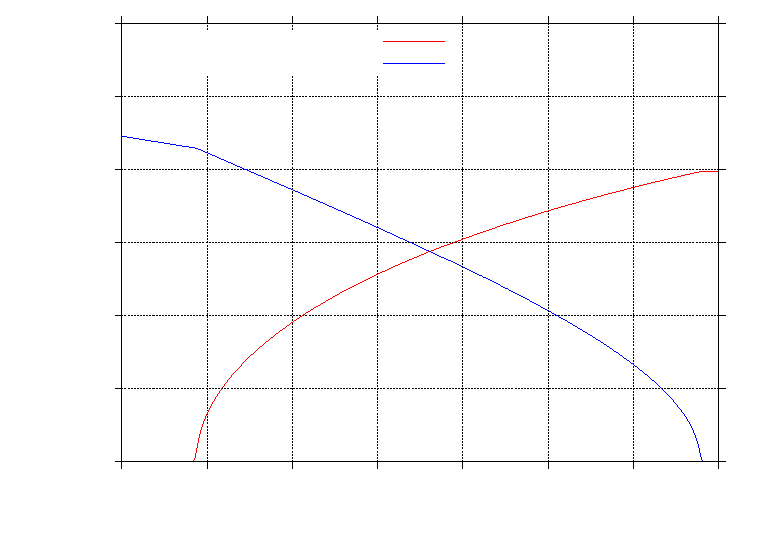
\includegraphics{ddepend}}%
    \gplfronttext
  \end{picture}%
\endgroup
  
\caption{The maximal pairings $\max_k\left[\Delta^{11}_k\right]$ and $\max_k\left[\Delta^{12}_k\right]$ in red and blue plotted as a function of the distance $d$ between the wires. For the used set of parameters $k_F\frac{\xi}{\sqrt{2}} = 0.95$. We hereby see, that the cross over from intrawire to interwire dominated pairing happens for $\frac{\sqrt{2}d}{\xi} \approx 0.6$. The small indent at $k_Fd = 0.59$ is a numerical effect. Parameters: $(n_Ba_B^3)^{1/3} = 0.01$, $(n_Ba_{BF}^3)^{1/3} = 0.11$, $l_t = 0$, $\frac{m_B}{m_F} = 7/40$, $\frac{n_F}{n_B^{1/3}} = 0.215$, $v_F/c_0 = 0.33$. }  
\label{fig.maximalpairingddepend}  
\end{center}    
\end{figure}

The figure only shows the maximal pairing $\max_k[\Delta_k]$. The same analysis also gives us, how the functional form of the pairings are altered as the distance $d$ is varied. This is summarized in figure \ref{fig.pairingkdependT0dvaried}. This explicitly shows, that the interwire pairing is even in $k$ and hence is a $s$-wave type pairing. We see, that it has its maximum value at $k=0$ as one might expect from the interwire induced interaction. Further, it shows no oscillatory behaviour, it simply decays exponentially for large values of $k$. The intrawire pairing is seen to have the same functional form as for the single wire, hence a $p$-wave type pairing. The overall behaviour of the pairings are seen to be independent of $d$. The interwire pairing is simply enhanced as $d$ decreases, vice versa for the intrawire pairing.  

\begin{figure} 
\begin{center}  
% GNUPLOT: LaTeX picture with Postscript
\begingroup
  \makeatletter
  \providecommand\color[2][]{%
    \GenericError{(gnuplot) \space\space\space\@spaces}{%
      Package color not loaded in conjunction with
      terminal option `colourtext'%
    }{See the gnuplot documentation for explanation.%
    }{Either use 'blacktext' in gnuplot or load the package
      color.sty in LaTeX.}%
    \renewcommand\color[2][]{}%
  }%
  \providecommand\includegraphics[2][]{%
    \GenericError{(gnuplot) \space\space\space\@spaces}{%
      Package graphicx or graphics not loaded%
    }{See the gnuplot documentation for explanation.%
    }{The gnuplot epslatex terminal needs graphicx.sty or graphics.sty.}%
    \renewcommand\includegraphics[2][]{}%
  }%
  \providecommand\rotatebox[2]{#2}%
  \@ifundefined{ifGPcolor}{%
    \newif\ifGPcolor
    \GPcolorfalse
  }{}%
  \@ifundefined{ifGPblacktext}{%
    \newif\ifGPblacktext
    \GPblacktexttrue
  }{}%
  % define a \g@addto@macro without @ in the name:
  \let\gplgaddtomacro\g@addto@macro
  % define empty templates for all commands taking text:
  \gdef\gplbacktext{}%
  \gdef\gplfronttext{}%
  \makeatother
  \ifGPblacktext
    % no textcolor at all
    \def\colorrgb#1{}%
    \def\colorgray#1{}%
  \else
    % gray or color?
    \ifGPcolor
      \def\colorrgb#1{\color[rgb]{#1}}%
      \def\colorgray#1{\color[gray]{#1}}%
      \expandafter\def\csname LTw\endcsname{\color{white}}%
      \expandafter\def\csname LTb\endcsname{\color{black}}%
      \expandafter\def\csname LTa\endcsname{\color{black}}%
      \expandafter\def\csname LT0\endcsname{\color[rgb]{1,0,0}}%
      \expandafter\def\csname LT1\endcsname{\color[rgb]{0,1,0}}%
      \expandafter\def\csname LT2\endcsname{\color[rgb]{0,0,1}}%
      \expandafter\def\csname LT3\endcsname{\color[rgb]{1,0,1}}%
      \expandafter\def\csname LT4\endcsname{\color[rgb]{0,1,1}}%
      \expandafter\def\csname LT5\endcsname{\color[rgb]{1,1,0}}%
      \expandafter\def\csname LT6\endcsname{\color[rgb]{0,0,0}}%
      \expandafter\def\csname LT7\endcsname{\color[rgb]{1,0.3,0}}%
      \expandafter\def\csname LT8\endcsname{\color[rgb]{0.5,0.5,0.5}}%
    \else
      % gray
      \def\colorrgb#1{\color{black}}%
      \def\colorgray#1{\color[gray]{#1}}%
      \expandafter\def\csname LTw\endcsname{\color{white}}%
      \expandafter\def\csname LTb\endcsname{\color{black}}%
      \expandafter\def\csname LTa\endcsname{\color{black}}%
      \expandafter\def\csname LT0\endcsname{\color{black}}%
      \expandafter\def\csname LT1\endcsname{\color{black}}%
      \expandafter\def\csname LT2\endcsname{\color{black}}%
      \expandafter\def\csname LT3\endcsname{\color{black}}%
      \expandafter\def\csname LT4\endcsname{\color{black}}%
      \expandafter\def\csname LT5\endcsname{\color{black}}%
      \expandafter\def\csname LT6\endcsname{\color{black}}%
      \expandafter\def\csname LT7\endcsname{\color{black}}%
      \expandafter\def\csname LT8\endcsname{\color{black}}%
    \fi
  \fi
    \setlength{\unitlength}{0.0500bp}%
    \ifx\gptboxheight\undefined%
      \newlength{\gptboxheight}%
      \newlength{\gptboxwidth}%
      \newsavebox{\gptboxtext}%
    \fi%
    \setlength{\fboxrule}{0.5pt}%
    \setlength{\fboxsep}{1pt}%
\begin{picture}(7200.00,5040.00)%
    \gplgaddtomacro\gplbacktext{%
      \csname LTb\endcsname%
      \put(946,767){\makebox(0,0)[r]{\strut{}$-0.6$}}%
      \csname LTb\endcsname%
      \put(946,1468){\makebox(0,0)[r]{\strut{}$-0.4$}}%
      \csname LTb\endcsname%
      \put(946,2170){\makebox(0,0)[r]{\strut{}$-0.2$}}%
      \csname LTb\endcsname%
      \put(946,2871){\makebox(0,0)[r]{\strut{}$0$}}%
      \csname LTb\endcsname%
      \put(946,3573){\makebox(0,0)[r]{\strut{}$0.2$}}%
      \csname LTb\endcsname%
      \put(946,4275){\makebox(0,0)[r]{\strut{}$0.4$}}%
      \csname LTb\endcsname%
      \put(946,4976){\makebox(0,0)[r]{\strut{}$0.6$}}%
      \csname LTb\endcsname%
      \put(1141,484){\makebox(0,0){\strut{}$-10$}}%
      \csname LTb\endcsname%
      \put(2541,484){\makebox(0,0){\strut{}$-5$}}%
      \csname LTb\endcsname%
      \put(3941,484){\makebox(0,0){\strut{}$0$}}%
      \csname LTb\endcsname%
      \put(5340,484){\makebox(0,0){\strut{}$5$}}%
      \csname LTb\endcsname%
      \put(6740,484){\makebox(0,0){\strut{}$10$}}%
    }%
    \gplgaddtomacro\gplfronttext{%
      \csname LTb\endcsname%
      \put(176,2871){\rotatebox{-270}{\makebox(0,0){\strut{}$\Delta_k/\epsilon_{F,0}$}}}%
      \put(3940,154){\makebox(0,0){\strut{}$k/k_F$}}%
      \csname LTb\endcsname%
      \put(5753,1820){\makebox(0,0)[r]{\strut{}$k_Fd = 0.575$}}%
      \csname LTb\endcsname%
      \put(5753,1600){\makebox(0,0)[r]{\strut{}$k_Fd = 0.585$}}%
      \csname LTb\endcsname%
      \put(5753,1380){\makebox(0,0)[r]{\strut{}$k_Fd = 0.595$}}%
      \csname LTb\endcsname%
      \put(5753,1160){\makebox(0,0)[r]{\strut{}$k_Fd = 0.610$}}%
      \csname LTb\endcsname%
      \put(5753,940){\makebox(0,0)[r]{\strut{}$k_Fd = 0.620$}}%
    }%
    \gplbacktext
    \put(0,0){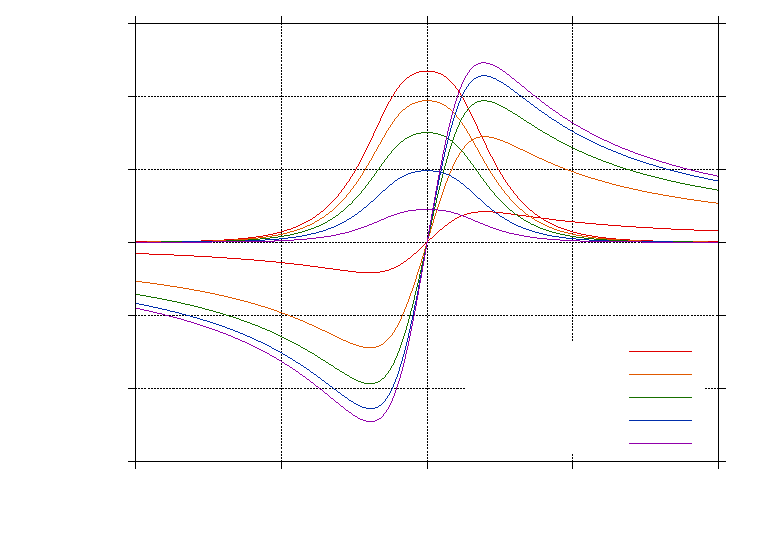
\includegraphics{Figures/twowires/Deltas1/kdepend}}%
    \gplfronttext
  \end{picture}%
\endgroup
  
\caption{The pairings $\Delta^{11}_k$ (odd) and $\Delta^{12}_k$ (even) plotted as a function of $k$. We see, that the functional behaviour is independent of $d$, and that there is a cross over between interwire and intrawire dominated pairing. The intrawire pairing is increased as $d$ increases. Vice versa for the interwire pairing. Parameters: $(n_Ba_B^3)^{1/3} = 0.01$, $(n_Ba_{BF}^3)^{1/3} = 0.11$, $l_t = 0$, $\frac{m_B}{m_F} = 7/40$, $\frac{n_F}{n_B^{1/3}} = 0.215$, $v_F/c_0 = 0.33$. }  
\label{fig.pairingkdependT0dvaried}  
\end{center}    
\end{figure}

The combined result of the two figures tells us the following. We are able to find a cross over region of interwire distances $d$, where both an interwire $s$-wave pairing and an intrawire $p$-wave pairing is present.

\section{Range of interaction dependency}
In this section we will investigate how the cross over from intrawire to interwire pairing depends on the range of the induced interaction. The range is roughly the condensate coherence length $\xi$, and it can be written unitlessly as:
\begin{equation}
k_F\frac{\xi}{\sqrt{2}} = \frac{\sqrt{\pi}}{4}\frac{1}{\sqrt{(n_Ba_B^3)^{1/3}}}\frac{n_F}{n_B^{1/3}}.
\end{equation}
It is physically reasonable, that for a longer interaction range, the interwire interaction will become comparable to the intrawire interaction at a larger critical distance $d_c$ between the wires. This is simply because the distance between the wires becomes less significant for a longer interaction range. Hence, we expect a monotonic increase of $d_c$ with $\xi$. However, it is not obvious, what the more detailed functional dependency might be.  

For the analysis, we will keep the Bose gas parameter $(n_Ba_B^3)^{1/3}$ constant and use the ratio of interparticle distances $n_F/n_B^{1/3}$ to vary the range of the interaction. The analysis is then performed in the following way. We start at a high value of $n_F/n_B^{1/3}$, and find the critical distance $d_c$ between the wires, where the maximal values of the interwire and intrawire pairings are equal. Then we decrease $n_F/n_B^{1/3}$ by a small amount. Since we expect $d_c$ to decrease with decreasing interaction range, we start an iteration over $d$ starting from $d = d_c$ going down with small decrements, until we reach a new value of $d_c$, where the pairings again are equal. This process is then repeated.

The outcome of the analysis is shown in figure \ref{fig.twowirescrossoverxidepend}. The figure shows the expected monotonic increase in the critical length $d_c$ with increasing coherence length, $\xi$. Further, it shows that $d_c$ saturates at some constant value $k_Fd_{c,s} = 0.677$, for $k_F\xi > 3$. This behaviour is nontrivial and it is not clear at the present stage, why it should saturate. 

\begin{figure} 
\begin{center}  
% GNUPLOT: LaTeX picture with Postscript
\begingroup
  \makeatletter
  \providecommand\color[2][]{%
    \GenericError{(gnuplot) \space\space\space\@spaces}{%
      Package color not loaded in conjunction with
      terminal option `colourtext'%
    }{See the gnuplot documentation for explanation.%
    }{Either use 'blacktext' in gnuplot or load the package
      color.sty in LaTeX.}%
    \renewcommand\color[2][]{}%
  }%
  \providecommand\includegraphics[2][]{%
    \GenericError{(gnuplot) \space\space\space\@spaces}{%
      Package graphicx or graphics not loaded%
    }{See the gnuplot documentation for explanation.%
    }{The gnuplot epslatex terminal needs graphicx.sty or graphics.sty.}%
    \renewcommand\includegraphics[2][]{}%
  }%
  \providecommand\rotatebox[2]{#2}%
  \@ifundefined{ifGPcolor}{%
    \newif\ifGPcolor
    \GPcolorfalse
  }{}%
  \@ifundefined{ifGPblacktext}{%
    \newif\ifGPblacktext
    \GPblacktexttrue
  }{}%
  % define a \g@addto@macro without @ in the name:
  \let\gplgaddtomacro\g@addto@macro
  % define empty templates for all commands taking text:
  \gdef\gplbacktext{}%
  \gdef\gplfronttext{}%
  \makeatother
  \ifGPblacktext
    % no textcolor at all
    \def\colorrgb#1{}%
    \def\colorgray#1{}%
  \else
    % gray or color?
    \ifGPcolor
      \def\colorrgb#1{\color[rgb]{#1}}%
      \def\colorgray#1{\color[gray]{#1}}%
      \expandafter\def\csname LTw\endcsname{\color{white}}%
      \expandafter\def\csname LTb\endcsname{\color{black}}%
      \expandafter\def\csname LTa\endcsname{\color{black}}%
      \expandafter\def\csname LT0\endcsname{\color[rgb]{1,0,0}}%
      \expandafter\def\csname LT1\endcsname{\color[rgb]{0,1,0}}%
      \expandafter\def\csname LT2\endcsname{\color[rgb]{0,0,1}}%
      \expandafter\def\csname LT3\endcsname{\color[rgb]{1,0,1}}%
      \expandafter\def\csname LT4\endcsname{\color[rgb]{0,1,1}}%
      \expandafter\def\csname LT5\endcsname{\color[rgb]{1,1,0}}%
      \expandafter\def\csname LT6\endcsname{\color[rgb]{0,0,0}}%
      \expandafter\def\csname LT7\endcsname{\color[rgb]{1,0.3,0}}%
      \expandafter\def\csname LT8\endcsname{\color[rgb]{0.5,0.5,0.5}}%
    \else
      % gray
      \def\colorrgb#1{\color{black}}%
      \def\colorgray#1{\color[gray]{#1}}%
      \expandafter\def\csname LTw\endcsname{\color{white}}%
      \expandafter\def\csname LTb\endcsname{\color{black}}%
      \expandafter\def\csname LTa\endcsname{\color{black}}%
      \expandafter\def\csname LT0\endcsname{\color{black}}%
      \expandafter\def\csname LT1\endcsname{\color{black}}%
      \expandafter\def\csname LT2\endcsname{\color{black}}%
      \expandafter\def\csname LT3\endcsname{\color{black}}%
      \expandafter\def\csname LT4\endcsname{\color{black}}%
      \expandafter\def\csname LT5\endcsname{\color{black}}%
      \expandafter\def\csname LT6\endcsname{\color{black}}%
      \expandafter\def\csname LT7\endcsname{\color{black}}%
      \expandafter\def\csname LT8\endcsname{\color{black}}%
    \fi
  \fi
    \setlength{\unitlength}{0.0500bp}%
    \ifx\gptboxheight\undefined%
      \newlength{\gptboxheight}%
      \newlength{\gptboxwidth}%
      \newsavebox{\gptboxtext}%
    \fi%
    \setlength{\fboxrule}{0.5pt}%
    \setlength{\fboxsep}{1pt}%
\begin{picture}(7200.00,5040.00)%
    \gplgaddtomacro\gplbacktext{%
    }%
    \gplgaddtomacro\gplfronttext{%
      \csname LTb\endcsname%
      \put(176,2871){\rotatebox{-270}{\makebox(0,0){\strut{}$k_Fd_c$}}}%
      \put(3874,154){\makebox(0,0){\strut{}$n_F/n_B^{1/3}$}}%
      \csname LTb\endcsname%
      \put(814,767){\makebox(0,0)[r]{\strut{}$0$}}%
      \csname LTb\endcsname%
      \put(814,1469){\makebox(0,0)[r]{\strut{}$0.2$}}%
      \csname LTb\endcsname%
      \put(814,2170){\makebox(0,0)[r]{\strut{}$0.4$}}%
      \csname LTb\endcsname%
      \put(814,2872){\makebox(0,0)[r]{\strut{}$0.6$}}%
      \csname LTb\endcsname%
      \put(814,3573){\makebox(0,0)[r]{\strut{}$0.8$}}%
      \csname LTb\endcsname%
      \put(814,4275){\makebox(0,0)[r]{\strut{}$1$}}%
      \csname LTb\endcsname%
      \put(814,4976){\makebox(0,0)[r]{\strut{}$1.2$}}%
      \csname LTb\endcsname%
      \put(1009,484){\makebox(0,0){\strut{}$0$}}%
      \csname LTb\endcsname%
      \put(1773,484){\makebox(0,0){\strut{}$0.2$}}%
      \csname LTb\endcsname%
      \put(2537,484){\makebox(0,0){\strut{}$0.4$}}%
      \csname LTb\endcsname%
      \put(3301,484){\makebox(0,0){\strut{}$0.6$}}%
      \csname LTb\endcsname%
      \put(4066,484){\makebox(0,0){\strut{}$0.8$}}%
      \csname LTb\endcsname%
      \put(4830,484){\makebox(0,0){\strut{}$1$}}%
      \csname LTb\endcsname%
      \put(5594,484){\makebox(0,0){\strut{}$1.2$}}%
      \csname LTb\endcsname%
      \put(6358,484){\makebox(0,0){\strut{}$1.4$}}%
      \put(1850,3924){\makebox(0,0)[l]{\strut{}Intrawire pairing only}}%
      \put(4142,2521){\makebox(0,0)[l]{\strut{}Interwire pairing only}}%
    }%
    \gplbacktext
    \put(0,0){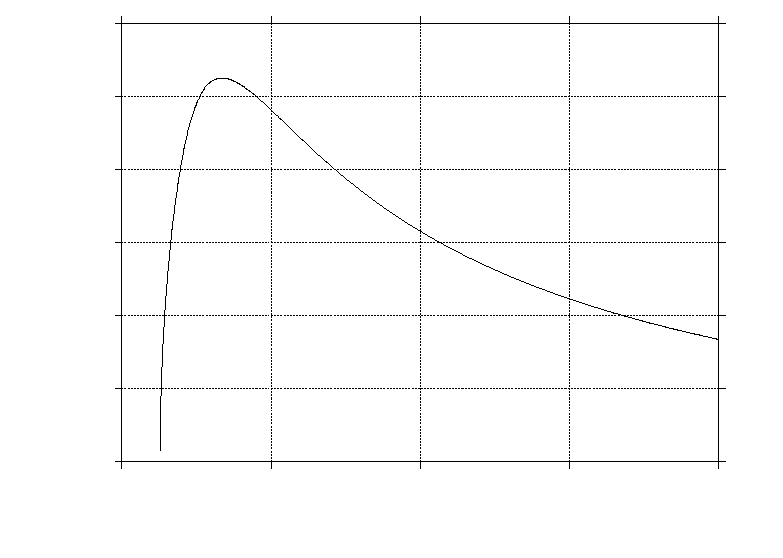
\includegraphics{Figures/twowires/Deltas3.1.3/nBdepend}}%
    \gplfronttext
  \end{picture}%
\endgroup
  
\caption{The critical distance $d_c$ plotted as a function of the coherence length $\xi$. A monotonic increase of $d_c$ with $\xi$ is observed. The plot is halted when $v_F = c_0$. Parameters: $(n_Ba_B^3)^{1/3} = 0.01$, $(n_Ba_{BF}^3)^{1/3} = 0.11$, $l_t = 0$, $\frac{m_B}{m_F} = 7/40$. }  
\label{fig.twowirescrossoverxidepend}  
\end{center}    
\end{figure}

Even though the range of the induced interaction is relatively long, $k_F\xi > 3$, the wires still have to be brought closer than $k_Fd = 0.7$ for the interwire pairing to kick in. This is \textit{not} in agreement with the intuitive idea given in the end of chapter \ref{Chapter8}, that the interwire interaction will become significant at a distance around the range of the interaction! The result of this section therefore calls for a deeper analysis. 

 


